% Chapter 3

\chapter{Research Methodology} % Main chapter title

\section{Introduction}
This section describes which research approach was chosen and why. Further, it elaborates, how the research approach is implemented and what work is done in the corresponding sections. 

\section{Research Design}
As research methodology experimental research was chosen. Experimental research typically focuses on systematically testing a hypothesis. It is often applied to research fields such as physics and chemistry but also psychology. In this research project, the hypothesis to test is formulated as the thesis statement (see section \ref{thesisstatement}).\\
\\
Experimental research knows five process steps. These are:

\begin{itemize}
	\item Awareness of the Problem
	\item Design of Experiments
	\item Experiments
	\item Evaluation
	\item Conclusion
\end{itemize}

In the following, it is outlined what will be done in the different process steps and how it is going to help answering the research question and test the thesis statement. Figure \ref{Thesis Map} illustrates the different steps.

\begin{figure}[h]
	\centering
	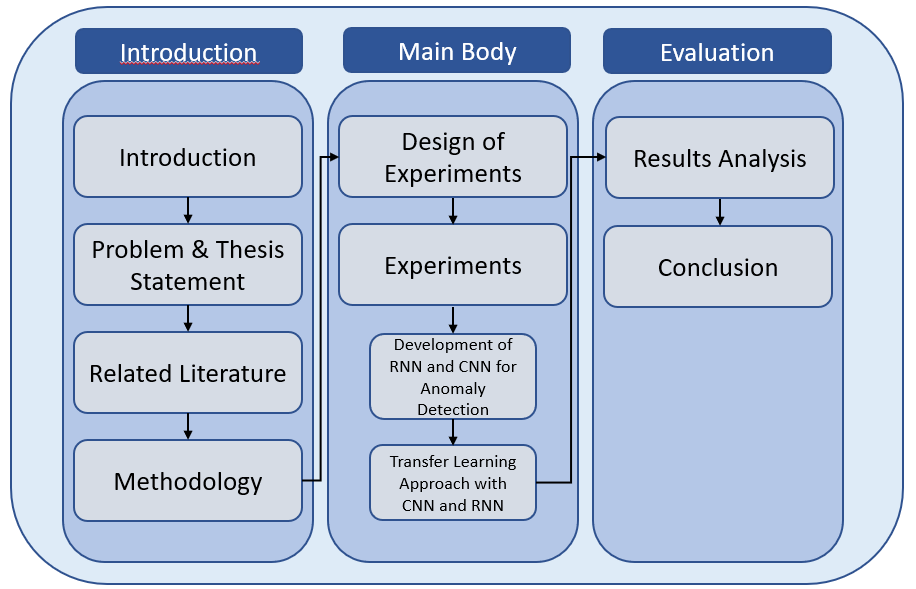
\includegraphics[scale=0.5]{Figures/Thesis Map}
	\decoRule
	\caption[Thesis Map]{Thesis Map \parencite{own}}
	\label{Thesis Map}
\end{figure}

\newpage
\subsection{Awareness of the Problem - Literature Review}
In this work, the literature review consists of two parts, background information presented in Section \ref{background} and the part Related Literature presented as Chapter \ref{relatedLiterature}. The reason for this split is to give insight on how neural networks and especially the derived architectures such as CNN and RNN work. A basic understanding of these two architectures is required to comprehend the problem and thesis statement presented in Sections \ref{Problem} and \ref{thesisstatement}. 

Further, the part Related Literature should deliver insights on how CNN and RNN are applied to detect anomalies. Where helpful, the publications investigated not only focus on detecting anomalies but also on related fields such as classification or prediction of time series. The investigated knowledge fields should serve as suggestions on how anomaly detection models can be set up. 

At last, to be able to answer the research question it is investigated how the different architectures, RNN and CNN, can be compared and what measures are important. 

\subsection{Experimental Design}
In this section, it is outlined how the experiments are designed. It is described how and why datasets are selected as well as which architecture principles are followed when designing the neural networks.

\subsubsection{Data Selection}
As explained in Section \ref{anomalies}, there are several types of anomalies, each of which is more or less difficult to identify. Appropriate data sets are suggested under the Section Experimental Design \ref{ExpDesign}. To perform experiments, at least three separate data sets are suggested. In Section Datasets \ref{Datasets}, it is further reasoned why the proposed datasets are chosen.
 
A careful selection of datasets is critical since it has a direct influence on how experiments must be designed. The datasets define whether a supervised approach may be employed or if only unsupervised methods can be utilized. Because both approaches will be examined, at least one of the datasets must be labeled. 

\subsubsection{Setup of Experiments}
The general setup of the experiments is detailed in the Section Setup of Experiments \ref{SetupOfExperiments}. As discussed in the section Related Literature \ref{relatedLiterature}, there are two basic methods for detecting anomalies: supervised and unsupervised. The Section Section Setup of Experiments \ref{SetupOfExperiments} describes how the neural network topologies must be created for each approach. 
   
Further, in Section \ref{SetupOfExperiments}, all global hyper-parameters are defined. Global hyper-parameters are parameters that must be explicitly defined rather than learnt and are valid across all experiments. The optimizer function and its accompanying parameters are an example of such a global parameter. 

\subsection{Experiments}
Finally, in the Chapter Experiments the proposed experimental setup is implemented. The experiments are only conducted on multivariate time series, since Braei and Wagner \parencite*{Braei2020} already issued a comprehensive study comparing different approaches for anomaly detection on univariate time series. 

In Chapter \ref{Experiments} Experiments, the various experiments are discussed. First, the dataset as well as the contained anomalies are introduced. Following that, the neural network architecture is described, including all hyperparameters that are not globally specified. Finally, the outcomes of the respective experiments are provided. Three experiments with datasets of various complexity are carried out in total.  


\subsection{Evaluation - Results Analysis}
The Chapter Results Analysis is dedicated to the examination of the previously achieved results. The results are compared using predefined metrics such as training time, inference time and F1-Score. Looking at these metrics helps to compare the neural network architectures and to determine whether CNN are actually superior to RNN when applied for anomaly detection. In addtion, insights learned from the experiments are presented and the usefulness of deep learning is ranked.

\subsection{Conclusion}
In the Chapter Conclusion, the research questions are addressed. Answering the research questions will provide an overview of the most significant findings from the experiments. Second, the thesis statement's insights are presented, which aid in determining whether the thesis statement is rejected or accepted. Finally, further research topics are suggested based on the findings of this study. 


